% ================================================================
% Design and Development of a Five-Degree-of-Freedom 3D Printer
% Complete, editable LaTeX proposal. Compile twice with pdfLaTeX.
% Keep the four PNG figures inside a folder named "figures".
% This is a proposal: targets and calculations are not test results.
% ================================================================
\documentclass[12pt,a4paper]{article}

% Page layout, mathematics, figures and multipage tables
\usepackage[margin=2.5cm]{geometry}
\usepackage{amsmath,amssymb}
\usepackage{graphicx}
\usepackage{float}
\usepackage{titlesec,needspace}
\usepackage{longtable,booktabs,array,calc}
\usepackage[hyphens]{url}
\usepackage[hidelinks]{hyperref}
\hypersetup{pdftitle={Design and Development of a Five-Degree-of-Freedom 3D Printer}}

\linespread{1.08}
\setlength{\parindent}{0pt}
\setlength{\parskip}{0.20em}
\setlength{\emergencystretch}{2em}
\titleformat{\section}{\large\bfseries}{\thesection}{1em}{}
\titleformat{\subsection}{\normalsize\bfseries}{\thesubsection}{1em}{}
\titlespacing*{\section}{0pt}{1.6ex plus 0.5ex minus 0.2ex}{0.7ex}
\titlespacing*{\subsection}{0pt}{1.3ex plus 0.4ex minus 0.2ex}{0.5ex}
\titlespacing*{\subsubsection}{0pt}{1.0ex plus 0.3ex minus 0.2ex}{0.4ex}
\setcounter{secnumdepth}{3}
\providecommand{\tightlist}{\setlength{\itemsep}{0pt}\setlength{\parskip}{0pt}}
\renewcommand{\labelitemi}{\ensuremath{\bullet}}

% ----------------- EDIT THESE TITLE-PAGE DETAILS -----------------
\newcommand{\thesistitle}{Design and Development of a Five-Degree-of-Freedom 3D Printer}
\newcommand{\thesisauthor}{[Student Name(s) and ID Number(s)]}
\newcommand{\thesisadvisor}{[Advisor Name]}
\newcommand{\thesisdate}{[Month Year]}
\newcommand{\thesisdepartment}{Department of Electromechanical Engineering}
\newcommand{\thesiscollege}{College of Engineering}
\newcommand{\thesisuniversity}{Addis Ababa Science and Technology University}
% ---------------------------------------------------------------

\begin{document}

\hypersetup{pageanchor=false}
\begin{titlepage}
  \centering
  \vspace*{1cm}
  {\Large\bfseries \thesistitle\par}
  \vspace{1.5cm}
  A Design of Mechatronics Thesis Proposal Submitted to the\\
  \thesisdepartment\par
  \vspace{1cm}
  {\bfseries \thesiscollege\\ \thesisuniversity\par}
  \vspace{1.5cm}
  {\bfseries By}\par
  \vspace{0.5cm}
  \thesisauthor\par
  \vspace{1.5cm}
  \textbf{Advisor:} \thesisadvisor\par
  \vspace{1cm}
  {\small\itshape Proposal draft: design targets and calculations are preliminary; experimental results
  are not yet available.\par}
  \vfill
  \thesisdate\\
  Addis Ababa, Ethiopia
\end{titlepage}
\hypersetup{pageanchor=true}
\pagenumbering{arabic}

% ---------------------- THESIS PROPOSAL -------------------------
\section*{Abstract}\label{abstract}

Conventional three-axis material-extrusion printers build mainly in a fixed orientation. Overhanging
  features may therefore require temporary supports, while curved surfaces can show a stair-step pattern.
  This thesis proposal presents the design and development of a five-degree-of-freedom (5-DOF)
  fused-filament-fabrication printer for laboratory-scale polymer parts. The proposed machine combines
  three Cartesian translations of a vertically oriented nozzle with a two-axis tilting and rotating build
  table. Three machine concepts are compared, and the Cartesian gantry with an A/C rotary table is
  selected using a weighted decision matrix. The study develops a preliminary mechanical architecture,
  coordinate transformation, actuator-sizing examples, a coordinated motion and temperature-control
  strategy, and a staged verification plan. A 150 mm \ensuremath{\times} 150 mm heated bed, a 0.4 mm
  nozzle, and polylactic acid filament are proposed as the initial test configuration. Validation will
  compare a conventional planar path with a feasible five-axis path for the same overhanging test part,
  alongside independent positioning, temperature and safety checks. Reduced support use and improved
  access are research objectives, not guaranteed outcomes; nozzle clearance, bed adhesion, rotary limits,
  software capability and material flow remain important constraints. The numerical calculations are
  design illustrations, and no prototype measurements or experimental results are claimed.

\textbf{Keywords:} five-degree-of-freedom printer; fused filament fabrication; tilting rotary table;
  nonplanar slicing; mechatronics; support reduction.

\clearpage
\section{Introduction}\label{introduction}

\subsection{Background of the Study}\label{background-of-the-study}

Additive manufacturing produces parts from digital descriptions through the successive addition of
  material. Fused filament fabrication (FFF) is a material-extrusion process in which a motor feeds
  thermoplastic filament into a heated nozzle, and the deposited material bonds to the previously placed
  material \cite{iso52900}. Its relatively accessible equipment and feedstock make it useful for
  prototypes, teaching aids and small functional parts.

A conventional Cartesian printer positions its nozzle along the \(X\), \(Y\) and \(Z\) directions while
  the deposition axis remains essentially fixed relative to the build plate. Most conventional slicers
  create flat, horizontal layers. On curved or shallow-sloping surfaces, these discrete layers can create
  visible steps; overhanging features can require support that consumes material and must later be
  removed. Strength and finish also depend on the material, deposition orientation, thermal history and
  other process parameters \cite{ahlers2019,nayyeri2022,tymrak2014}.

In five-axis printing, two additional rotations change the orientation between the nozzle and the part.
  They can enable selected inclined or curved paths and reduce support for some geometries, but introduce
  coupled motion, collision, calibration, extrusion and software problems
  \cite{shen2018,isa2019,hong2022,han2025}. This project treats the printer as an integrated mechanical,
  electronic, thermal and control system rather than as a conventional printer with two motors added.

\subsection{Problem Statement}\label{problem-statement}

A three-axis printer with a fixed build orientation has limited access to features that extend beyond
  material already deposited. Support structures can increase material consumption and post-processing,
  and planar layers may not be well aligned with a desired surface. A five-axis machine may address some
  of these limitations, but a successful design must also coordinate rotary and linear movements,
  compensate for the position of the rotary pivot, avoid collisions with the part and fixtures, manage
  cables on the moving table, and maintain a stable extrusion rate. Five-axis software and additional
  components can also make the system difficult to assemble and validate in an educational laboratory.

The problem addressed by this study is therefore how to design and evaluate an educational 5-DOF FFF
  printer that combines attainable mechanical construction with a defined kinematic model, safe
  coordinated motion and a reproducible comparison with ordinary planar printing. The project does not
  assume that every overhang can be printed without support or that an untested machine is more accurate
  than an existing printer.

\subsection{Objectives of the Study}\label{objectives-of-the-study}

\subsubsection{General Objective}\label{general-objective}

To design, model, develop and experimentally evaluate a laboratory-scale five-degree-of-freedom 3D
  printer capable of coordinated material extrusion on selected inclined and curved paths.

\subsubsection{Specific Objectives}\label{specific-objectives}

\begin{itemize}
\tightlist
\item
  To identify the functional, workspace, safety and performance requirements of a 5-DOF FFF printer.
\item
  To develop three five-axis concepts and select one using a transparent evaluation matrix.
\item
  To size the principal actuators and structure using stated load assumptions, and develop a detailed 3D
  CAD model.
\item
  To analyse the frame and rotary supports by hand calculations and finite element analysis (FEA).
\item
  To derive and verify the kinematic transformations between a rotating part and the Cartesian nozzle.
\item
  To develop a coordinated motion, filament-feed and temperature-control architecture with appropriate
  safety interlocks.
\item
  To fabricate and calibrate a prototype, then test positioning, temperature control and representative
  print quality.
\item
  To compare support material and print completion for a selected overhanging part made with three-axis
  and five-axis paths.
\end{itemize}

\subsection{Scope of the Study}\label{scope-of-the-study}

The intended prototype uses one nozzle, 1.75 mm diameter polylactic acid (PLA) filament, three linear
  positioning axes, and a build table with one bounded tilt axis and one bounded rotation axis. The work
  covers concept selection, CAD, preliminary analysis, motion planning, a laboratory prototype and bench
  testing. A conventional planar print at zero tilt is the comparison baseline; indexed 3+2 printing and
  a small continuous five-axis path will be investigated in stages.

The study does not cover metal or composite printing, multiple materials, industrial certification,
  arbitrary part geometries, commercial production, or a universal automatic five-axis slicer. The
  specified dimensions and performance limits are design targets, not demonstrated capabilities. A part
  must also satisfy the mass, clearance, adhesion, motion and temperature limits in every planned
  orientation.

\subsection{Significance of the Study}\label{significance-of-the-study}

The study provides a structured design example for students integrating mechanics, electronics, control,
  CAD and manufacturing. If experimentally verified, the proposed platform could allow local
  investigation of nonplanar paths and support reduction on suitable small parts. The documented
  coordinate convention, preliminary calculations and test procedure are intended to make the design
  easier to reproduce and improve. The degree of any benefit must be established by the proposed
  measurements rather than assumed from the additional axes.

\subsection{Research Questions}\label{research-questions}

\begin{enumerate}
\def\labelenumi{\arabic{enumi}.}
\tightlist
\item
  Can an A/C table and a Cartesian nozzle be coordinated to maintain a specified tool position and
  orientation within the proposed workspace?
\item
  Can a selected overhanging PLA test piece be completed with less support material than its planar
  baseline, without unacceptable dimensional error or a lower completion rate?
\item
  Which practical limitations in calibration, collision clearance, bed adhesion and thermal behaviour
  restrict the useful orientations?
\end{enumerate}

\clearpage
\section{Literature Review}\label{literature-review}

\textbf{Terminology and process.} ISO/ASTM 52900:2021 defines additive-manufacturing terminology and
  identifies material extrusion as a process category \cite{iso52900}. In this proposal, FFF denotes
  filament-fed material extrusion; the five degrees of freedom refer to the relative tool pose, not to
  the filament-feed actuator.

\textbf{Machine and part design.} Wulle et al.~discuss the relationship between workpiece and machine
  design for multi-axis FFF \cite{wulle2017}. Their work illustrates that the part, printhead and machine
  arrangement must be considered together. Consequently, the proposed design treats the printed part,
  fixture and printhead as collision bodies rather than relying on axis travel alone.

\textbf{Five-axis machine and process characteristics.} Shen et al.~describe a five-axis FFF machine and
  printing methods, and examine extrusion behaviour associated with different printing modes
  \cite{shen2018}. This supports including both motion and flow control in the proposed system. Their
  published results do not establish the performance of the new concept described here.

\textbf{Curved-layer planning.} Isa and Lazoglu propose five-axis planning based on transition layers for
  freeform parts \cite{isa2019}. Their work shows the importance of connecting layer geometry with
  machine orientation. A practical limitation for the present project is that feasible paths must also
  respect its comparatively small tilt range and finite rotary travel.

\textbf{Accessible implementation.} Hong et al.~present Open5x, an accessible five-axis printer and
  conformal-slicing workflow \cite{hong2022}. The work demonstrates a useful hardware-and-software
  direction for educational systems, but its implementation cannot be assumed to operate an arbitrary
  machine without adapting geometry, firmware, calibration and safety checks.

\textbf{Nonplanar slicing and clearance.} Ahlers et al.~combine planar and nonplanar layers and consider
  printhead collisions on a three-axis printer \cite{ahlers2019}. Their work is not a five-axis machine,
  but it is relevant because a curved path can collide with previously deposited material even without
  rotating the table. Nayyeri et al.~review planar and nonplanar slicing approaches and their trade-offs
  \cite{nayyeri2022}. Together, these studies motivate a conservative, geometry-specific planner rather
  than assuming that a conventional slicer automatically produces safe five-axis commands.

\textbf{Overhangs and mechanical properties.} Han et al.~investigate a five-axis method for selected
  overhanging parts \cite{han2025}; reductions reported for their specimens and equipment should not be
  transferred to this proposed machine. Tymrak et al.~characterize tensile properties of printed polymer
  specimens under realistic printing conditions \cite{tymrak2014}. Their work motivates reporting
  material and process parameters, but this proposal does not claim that five-axis motion alone improves
  strength.

\textbf{Research gap addressed.} Published multi-axis examples establish feasibility for particular
  systems and parts. A useful educational contribution is a fully specified, bounded A/C table design
  that links axis conventions and pivot compensation to actuator sizing, a safe controller, and a
  repeatable comparison against its own three-axis baseline. Whether it performs as intended remains to
  be tested.

\clearpage
\section{Methodology and Design Workflow}\label{methodology-and-design-workflow}

The work will proceed through requirements definition, concept selection, analytical sizing, CAD and FEA,
  controller and toolpath implementation, fabrication, calibration and controlled testing. At each stage
  the requirements will be reviewed; failed checks will lead to redesign before the next stage. Figures
  are original conceptual schematics and are not construction drawings.

\subsection{Proposed Conceptual Designs}\label{proposed-conceptual-designs}

\subsubsection{Concept 1: Cartesian Gantry with a Tilting Print
  Head}\label{concept-1-cartesian-gantry-with-a-tilting-print-head}

A Cartesian gantry translates the printhead in three directions, while an A/B rotary wrist changes nozzle
  direction over a fixed bed. The stationary bed can support relatively heavy parts without rotating the
  heater cable or the part. However, the hot end, feed system and cables move with the wrist, adding
  moving mass and increasing the need for tip-offset compensation. Compact wrist joints and sufficient
  nozzle clearance are important design challenges.

\begin{figure}[H]
\centering
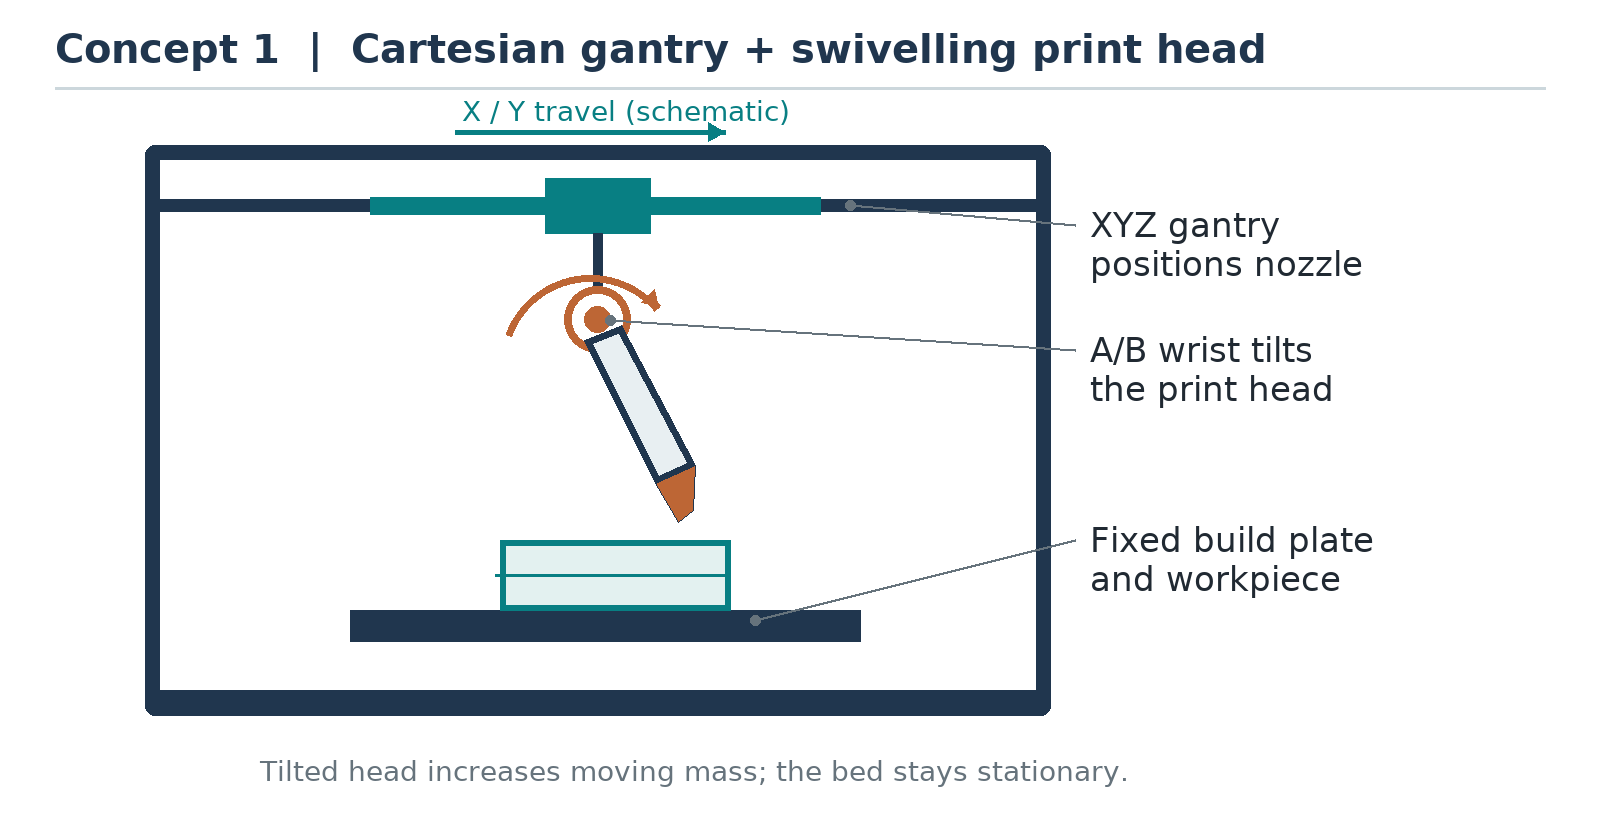
\includegraphics[width=0.9\linewidth,height=\textheight,keepaspectratio]{figures/concept_1_tilting_head.png}
\caption{Concept 1: Three Cartesian translations with a two-axis printhead wrist. The figure is schematic
  and not to scale.}
\end{figure}

\subsubsection{Concept 2: Cartesian Gantry with a Tilting and Rotating
  Table}\label{concept-2-cartesian-gantry-with-a-tilting-and-rotating-table}

A Cartesian gantry positions a vertical nozzle. Below it, a trunnion tilts the table about a fixed
  horizontal A axis; the C axis rotates the plate about its own normal. The part moves with the plate, so
  the nozzle orientation relative to the part changes even though the nozzle remains vertical in the
  machine frame. The arrangement uses a relatively simple printhead but requires a rigid table, a bounded
  flexible heater harness, secure part adhesion and careful rotary-pivot calibration.

\begin{figure}[H]
\centering
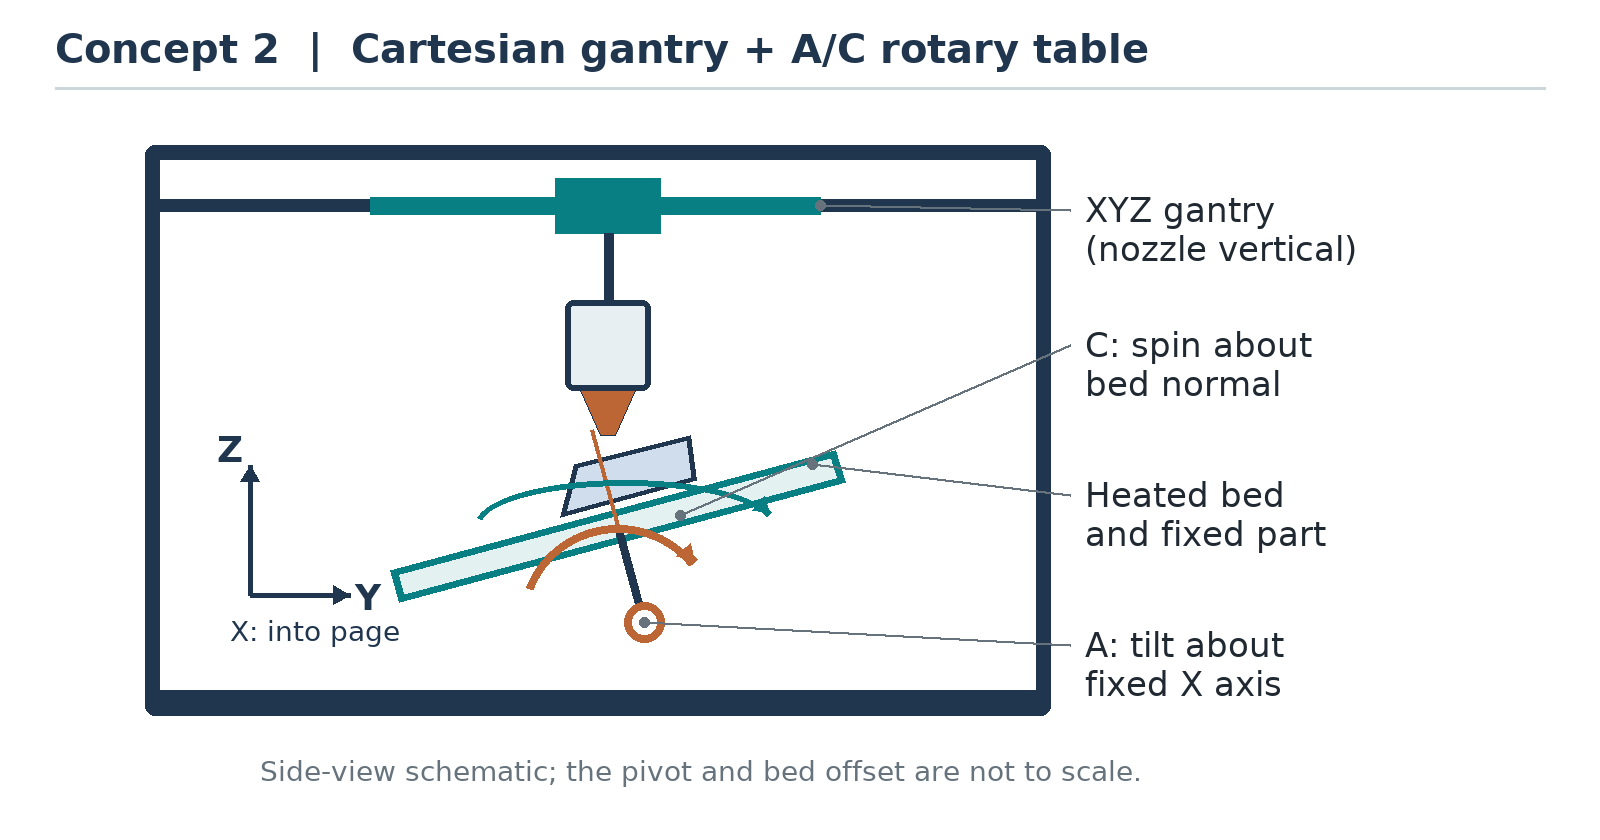
\includegraphics[width=0.9\linewidth,height=\textheight,keepaspectratio]{figures/concept_2_tilting_table.png}
\caption{Concept 2: A Cartesian nozzle and an A/C table. The A-axis pivot and the C-axis rotation are
  schematic.}
\end{figure}

\subsubsection{Concept 3: Delta Gantry with a Tilting and Rotating
  Table}\label{concept-3-delta-gantry-with-a-tilting-and-rotating-table}

Three coordinated tower carriages and parallel links position the nozzle in \(X\), \(Y\) and \(Z\); an
  A/C table provides the other two orientation degrees of freedom. The delta arrangement can keep the
  moving printhead light. However, its nonlinear position mapping, link calibration and collision checks
  make the control and assembly more demanding for this initial project. As in Concept 2, the table and
  payload must be moved safely.

\begin{figure}[H]
\centering
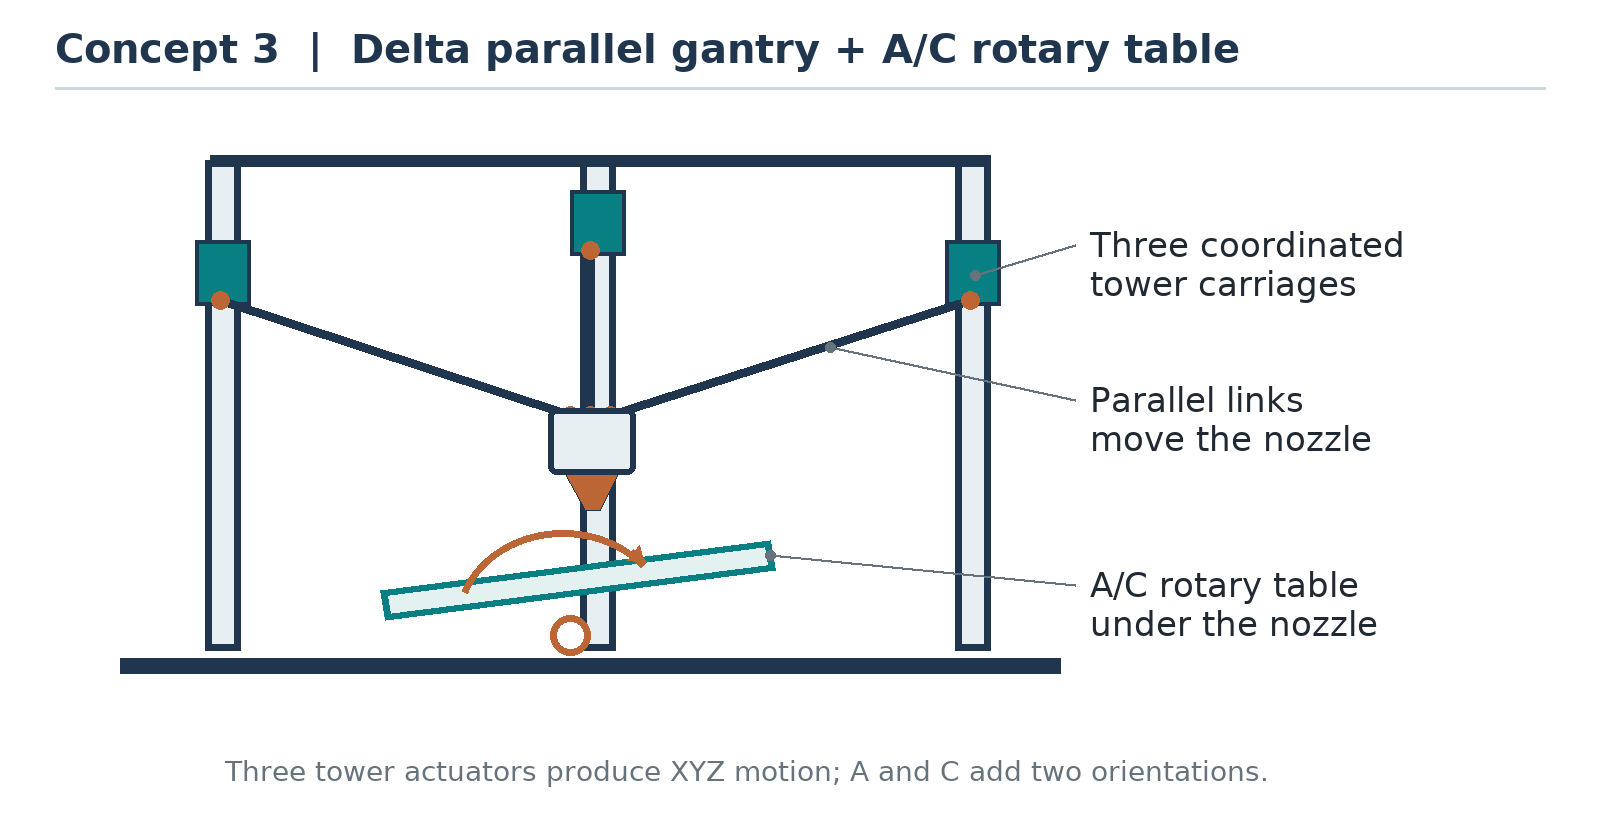
\includegraphics[width=0.9\linewidth,height=\textheight,keepaspectratio]{figures/concept_3_delta_table.png}
\caption{Concept 3: Three delta-tower actuators provide Cartesian tool position, while the A/C table
  provides orientation.}
\end{figure}

\subsection{Concept Evaluation and Selection}\label{concept-evaluation-and-selection}

The alternatives are scored from 1 (least favourable) to 5 (most favourable) for the stated
  educational-laboratory priorities. Weights total 100\%. The weighted score is the sum of weight
  \ensuremath{\times} score divided by 100; it therefore ranges from 1 to 5. The numbers are preliminary
  engineering judgments, not experimental measurements or procurement quotes.

\begingroup
\footnotesize
\setlength{\tabcolsep}{4pt}
\renewcommand{\arraystretch}{1.12}
\begin{longtable}[]{@{}
  >{\raggedright\arraybackslash}p{(\linewidth - 8\tabcolsep) * \real{0.3649}}
  >{\raggedleft\arraybackslash}p{(\linewidth - 8\tabcolsep) * \real{0.1081}}
  >{\raggedleft\arraybackslash}p{(\linewidth - 8\tabcolsep) * \real{0.1757}}
  >{\raggedleft\arraybackslash}p{(\linewidth - 8\tabcolsep) * \real{0.1757}}
  >{\raggedleft\arraybackslash}p{(\linewidth - 8\tabcolsep) * \real{0.1757}}@{}}
\caption{Preliminary concept-selection matrix.}\tabularnewline
\toprule\noalign{}
\begin{minipage}[b]{\linewidth}\raggedright
Criterion
\end{minipage} & \begin{minipage}[b]{\linewidth}\raggedleft
Weight
\end{minipage} & \begin{minipage}[b]{\linewidth}\raggedleft
1: Tilting head
\end{minipage} & \begin{minipage}[b]{\linewidth}\raggedleft
2: A/C table
\end{minipage} & \begin{minipage}[b]{\linewidth}\raggedleft
3: Delta + table
\end{minipage} \\
\midrule\noalign{}
\endfirsthead
\toprule\noalign{}
\begin{minipage}[b]{\linewidth}\raggedright
Criterion
\end{minipage} & \begin{minipage}[b]{\linewidth}\raggedleft
Weight
\end{minipage} & \begin{minipage}[b]{\linewidth}\raggedleft
1: Tilting head
\end{minipage} & \begin{minipage}[b]{\linewidth}\raggedleft
2: A/C table
\end{minipage} & \begin{minipage}[b]{\linewidth}\raggedleft
3: Delta + table
\end{minipage} \\
\midrule\noalign{}
\endhead
\bottomrule\noalign{}
\endlastfoot
Expected cost and component availability & 25\% & 2 & 4 & 2 \\
Mechanical simplicity and stiffness & 25\% & 2 & 4 & 2 \\
Part access and usable workspace & 15\% & 4 & 3 & 3 \\
Calibration and control integration & 20\% & 3 & 3 & 2 \\
Maintenance and modification & 15\% & 3 & 4 & 3 \\
\textbf{Weighted score out of 5} & \textbf{100\%} & \textbf{2.65} & \textbf{3.65} & \textbf{2.30} \\
\end{longtable}
\endgroup

\textbf{Selection and justification.} Concept 2 is selected because its Cartesian mechanism and vertical
  hot end are relatively straightforward to construct and maintain. Concept 1 scores better for keeping
  the bed stationary and accessing the part, but has a heavier articulated head. Concept 3 has additional
  delta calibration and control complexity. The selected concept still needs custom five-axis motion
  planning, collision checking and table calibration; its higher score is relative, not proof of
  feasibility. Scores should be reconsidered if component quotations or CAD/FEA show that the assumed
  table mass, stiffness or costs are unattainable.

\subsection{Design Basis and Mechanical Analysis}\label{design-basis-and-mechanical-analysis}

\subsubsection{Preliminary Requirements}\label{preliminary-requirements}

The following values are preliminary design targets used to make the calculations and tests specific.
  They are not verified specifications. All dimensions are subject to detailed CAD and a swept-volume
  check, especially when the bed tilts or turns.

% Keep this short requirements table together on a page.
\Needspace{240pt}
\begingroup
\footnotesize
\setlength{\tabcolsep}{4pt}
\renewcommand{\arraystretch}{1.12}
\begin{longtable}[]{@{}
  >{\raggedright\arraybackslash}p{(\linewidth - 2\tabcolsep) * \real{0.2969}}
  >{\raggedright\arraybackslash}p{(\linewidth - 2\tabcolsep) * \real{0.7031}}@{}}
\caption{Initial design requirements and operating assumptions.}\tabularnewline
\toprule\noalign{}
\begin{minipage}[b]{\linewidth}\raggedright
Parameter
\end{minipage} & \begin{minipage}[b]{\linewidth}\raggedright
Proposed design basis
\end{minipage} \\
\midrule\noalign{}
\endfirsthead
\toprule\noalign{}
\begin{minipage}[b]{\linewidth}\raggedright
Parameter
\end{minipage} & \begin{minipage}[b]{\linewidth}\raggedright
Proposed design basis
\end{minipage} \\
\midrule\noalign{}
\endhead
\bottomrule\noalign{}
\endlastfoot
Process and feedstock & Single-nozzle FFF; 1.75 mm PLA filament \\
Printhead & Vertical nozzle, 0.4 mm diameter; initial layer height 0.20 mm \\
Bed and zero-tilt working envelope & 150 mm \ensuremath{\times} 150 mm heated bed; target up to 150 mm
  part height at A = C = 0, before fixture and collision deductions \\
Cartesian nozzle travel & Target X and Y: \ensuremath{-}125 to +125 mm; Z: 0 to 250 mm, measured from the
  rotary pivot \\
Rotary motion & A about fixed X: \ensuremath{-}30\ensuremath{^\circ} to +30\ensuremath{^\circ}; C about
  bed normal: \ensuremath{-}170\ensuremath{^\circ} to +170\ensuremath{^\circ} \\
Moving table and payload & At most 2.0 kg total rotating/tilting assembly, including at most 0.5 kg of
  part and attached fixtures combined \\
Process starting point & 30 mm/s part-relative print speed; nozzle 200 \ensuremath{^\circ}C; bed 55
  \ensuremath{^\circ}C, subject to filament and component limits \\
Machine frame & Approximate external target 450 mm \ensuremath{\times} 450 mm \ensuremath{\times} 550 mm;
  verify after detailed layout \\
\end{longtable}
\endgroup

The full zero-tilt envelope is not promised at nonzero angles: a tilted bed, part or fixture may leave
  the Cartesian range or collide with the nozzle and frame. The volume and 0.5 kg payload limit are
  simultaneous limits, not a claim that a solid object filling the whole volume is permitted. The C-axis
  range is bounded to protect the bed wiring; it is not continuous rotation. Mechanical stops,
  appropriately placed switches, software limits and a tested service loop will be provided. Planned
  moves will not wrap through a limit; if needed the head will retract and the table will unwind through
  a safe path.

\subsubsection{Frame and Linear Drives}\label{frame-and-linear-drives}

The proposed frame uses aluminium sections, guided Cartesian axes and a vertically moving gantry
  supported by a lead screw. An illustrative X-axis calculation assumes a moving mass of 1.2 kg,
  acceleration of 0.5 m/s\textsuperscript{2}, resistance of 5 N, an overall belt-drive efficiency of 0.80
  and a factor of 2 on calculated torque. A 20-tooth, 2 mm-pitch pulley has pitch radius \(r = 40/(2\pi)
  = 6.37\) mm. Thus:

\[
F_x = ma + F_f = (1.2)(0.5) + 5 = 5.6\ \mathrm{N}
\]

\[
T_{x,\mathrm{design}} = \frac{2F_xr}{\eta} = \frac{2(5.6)(0.00637)}{0.80} \approx 0.089\ \mathrm{N\,m}.
\]

For the Z drive, a 3.0 kg lifted gantry, the same acceleration, an 8 mm lead screw and 0.30 estimated
  efficiency give \(F_z = 3(9.81 + 0.5) = 30.93\) N. With a factor of 2, the required motor torque for
  one directly driven screw is:

\[
T_{z,\mathrm{design}}=\frac{2F_z L}{2\pi\eta}=\frac{2(30.93)(0.008)}{2\pi(0.30)}\approx 0.263\
  \mathrm{N\,m}.
\]

The screw lead \(L\) is the axial travel per revolution, not necessarily its thread pitch. These values
  exclude unmeasured joint friction and shocks. Motor selection must use the available torque at the
  required speed and temperature, not holding torque alone; both drives must be checked with real
  components. Z-axis back-driving must also be assessed, with a brake or other positive restraint if
  needed when power is removed.

As a first stiffness estimate, model a 350 mm simply supported aluminium rectangular tube with a centred
  15 N load, elastic modulus 69,000 N/mm\textsuperscript{2}, outside section 20 mm \ensuremath{\times} 40
  mm, and 2 mm wall thickness. With the 40 mm dimension vertical, the second moment of area and ideal
  mid-span deflection are:

\[
I=\frac{20(40)^3-16(36)^3}{12}=44{,}459\ \mathrm{mm^4}, \qquad
\delta=\frac{FL^3}{48EI}\approx 0.0044\ \mathrm{mm}.
\]

The corresponding ideal bending stress at the outer surface is approximately 0.59 MPa. This idealized
  beam is only a preliminary check: actual extrusions, holes, joints, supports and moving loads differ.
  The CAD/FEA model will include the real section, fasteners, rotary brackets and expected load cases; it
  will check mesh convergence, stress against the selected material and a provisional 0.10 mm static
  frame-deflection target. Contact, vibration and thermal movement must be assessed separately.

\subsubsection{Rotary-Table Sizing}\label{rotary-table-sizing}

Assume the complete tilted assembly has mass \(m=2.0\) kg, and its centre of mass has a worst-case
  perpendicular lever arm of 0.060 m about A. With estimated rotational inertia \(J_A=0.020\)
  kg\ensuremath{\cdot}m\textsuperscript{2}, angular acceleration \(\alpha_A=0.50\)
  rad/s\textsuperscript{2}, and friction torque of 0.15 N\ensuremath{\cdot}m, the required A-axis output
  torque with factor 2 is:

\[
T_{A,\mathrm{out}}=2(mgr+J_A\alpha_A+T_f)
=2(2.0\times9.81\times0.060+0.020\times0.50+0.15)
\approx 2.67\ \mathrm{N\,m}.
\]

For a 10:1 reduction and estimated 0.70 efficiency, the motor must deliver approximately
  \(2.67/(10\times0.70)=0.38\) N\ensuremath{\cdot}m at the operating speed. A motor nominally rated 0.8
  N\ensuremath{\cdot}m holding torque is only a candidate: its running torque, reducer rating, heating,
  bearing loads and mounting stiffness must be verified.

For C, suppose the moving assembly has up to 0.020 m radial mass eccentricity, maximum A tilt
  30\ensuremath{^\circ}, \(J_C=0.010\) kg\ensuremath{\cdot}m\textsuperscript{2}, angular acceleration
  0.50 rad/s\textsuperscript{2} and friction 0.10 N\ensuremath{\cdot}m. The conservative gravity moment
  about C is \(mg(0.020)\sin30^\circ=0.196\) N\ensuremath{\cdot}m. Including inertia and a factor of 2
  gives \(T_{C,\mathrm{out}}=2(0.196+0.005+0.10)=0.60\) N\ensuremath{\cdot}m. A 5:1 reducer at 0.80
  efficiency requires about 0.15 N\ensuremath{\cdot}m at the motor. These are assumed loads; cable
  forces, acceleration transients and the actual centre of mass must be measured or bounded. A normally
  engaged A-axis brake or equivalent positive restraint is required; the design will not rely solely on
  gearbox self-locking.

\subsection{Kinematic Model and Workspace}\label{kinematic-model-and-workspace}

\subsubsection{Coordinate Convention}\label{coordinate-convention}

Let the fixed machine frame be \((X,Y,Z)\), with \(Z\) upward. Let \(O\) be the intersection of the
  horizontal A-axis pivot line and the C-axis centreline. The part frame is attached to the rotating bed;
  its origin is the centre of the top build surface when the table is level. For the preliminary model
  the surface centre is \(h=20\) mm along the C axis from \(O\). Let \((u,v,w)\) be a point measured in
  the part frame from that surface centre. A positive A rotation follows the right-hand rule about fixed
  \(X\), and positive C rotation follows the right-hand rule about the local bed normal. Angles are
  expressed consistently in radians inside calculations.

The table rotation from the part frame to the machine frame is \(R=R_x(a)R_z(c)\). Assuming the commanded
  Cartesian coordinates describe the nozzle tip itself, the world-frame target is:

\[
\mathbf{p}_w = \mathbf{O} + R_x(a)R_z(c)
\begin{bmatrix}u\\v\\w+h\end{bmatrix}.
\]

With \(O\) as the Cartesian origin, the corresponding commanded coordinates are:

\[
x=u\cos c-v\sin c,
\]

\[
y=(u\sin c+v\cos c)\cos a-(w+h)\sin a,
\]

\[
z=(u\sin c+v\cos c)\sin a+(w+h)\cos a.
\]

Actual machines may have nonintersecting pivots, tool-tip offsets, gantry nonorthogonality and a
  different value of \(h\); these require calibration and an updated transform. The equations describe
  geometry, not proof that the nozzle body or table will clear the part.

\subsubsection{Orientation, Inverse Mapping and Numerical
  Check}\label{orientation-inverse-mapping-and-numerical-check}

The nozzle points toward the work along machine \(-Z\). Define the desired \emph{outward} tool-axis
  direction \(\mathbf{d}_p\) in the part frame as the direction from the nozzle tip away from the part;
  the corresponding machine-frame direction is \(+Z\). Therefore:

\[
\mathbf{d}_p=R^T\begin{bmatrix}0\\0\\1\end{bmatrix}
=\begin{bmatrix}\sin a\sin c\\\sin a\cos c\\\cos a\end{bmatrix}.
\]

For a unit direction \((d_x,d_y,d_z)\) away from the singularity, one inverse solution is
  \(a_1=\operatorname{atan2}(\sqrt{d_x^2+d_y^2},d_z)\) and \(c_1=\operatorname{atan2}(d_x,d_y)\). An
  equivalent orientation branch is \(a_2=-a_1\), \(c_2=c_1\pm180^\circ\) after appropriate angle
  normalization. The planner will select a continuous, physically reachable branch and reject directions
  or transitions outside A/C limits. At \(a=0\), \(c\) is indeterminate from the direction alone: keep
  the previous C angle unless the planned in-plane orientation requires a safe change. Near this
  singularity, limit rotary speed and plan continuity explicitly.

For an arithmetic check, use \((u,v,w)=(40,30,20)\) mm, \(h=20\) mm, \(a=20^\circ\) and \(c=30^\circ\).
  The equations give \((x,y,z)\approx(19.64,29.53,53.31)\) mm and
  \(\mathbf{d}_p\approx(0.1710,0.2962,0.9397)\). The inverse equations recover \(a=20^\circ\) and
  \(c=30^\circ\) on the positive-A branch. This is a mathematical example only, not a measured machine
  position.

A candidate pose is rejected if any axis exceeds its limit or if the head, printed geometry, clamps,
  table, frame or cable envelope collides during the move. For example, at \(a=30^\circ\), \(c=0^\circ\),
  the point \((u,v,w)=(0,-75,150)\) mm with \(h=20\) mm would require \(y\approx-150\) mm, outside the
  proposed \(-125\) to \(+125\) mm Y travel. Thus even a point within the nominal level-bed volume may be
  unreachable when tilted.

\subsection{System Dynamics and Control Strategy}\label{system-dynamics-and-control-strategy}

A general dynamic model for the five pose coordinates \(\mathbf{q}=[x,y,z,a,c]^T\) can be written as:

\[
M(\mathbf{q})\ddot{\mathbf{q}} + C(\mathbf{q},\dot{\mathbf{q}})\dot{\mathbf{q}} + g(\mathbf{q}) +
  B\dot{\mathbf{q}} = \boldsymbol{\tau}.
\]

Here \(M\) is the inertia matrix, \(C\) represents velocity-dependent coupling, \(g\) is the generalized
  gravity load, \(B\) represents approximate viscous losses, and \(\boldsymbol{\tau}\) contains
  generalized actuator forces and torques referred to the axes. The moving bed and part make the rotary
  loads configuration-dependent. An initial A-axis approximation for tuning is \(J_A\ddot a+b_A\dot
  a+mgd\sin(a+\phi)=T_{A,\mathrm{out}}\), where \(d\) and \(\phi\) describe the centre-of-mass offset and
  its reference angle. Parameters must be identified from the completed assembly; backlash and nonlinear
  friction are not represented by this simple model.

The motion controller must support simultaneous interpolated \(X,Y,Z,A,C\) motion \textbf{and} a
  synchronized extruder channel \(E\), together with configurable limits and the intended feed-time
  semantics. This is six actuated channels but five tool-pose degrees of freedom: \(E\) meters material
  and does not independently position or orient the nozzle. Standard three-axis slicer output or a
  controller merely exposing extra pins is not sufficient. The selected controller and postprocessor must
  be demonstrated together before hardware procurement is finalized.

Cartesian and extruder stepper drives may initially be open-loop, with homing switches; their commanded
  step counts are not proof of actual position. Output-side A/C encoders and compatible closed-loop
  drives are proposed to monitor rotary motion and permit appropriate position/velocity-loop tuning. The
  heater controller will use thermistor feedback and guarded PID or PI temperature control, with
  anti-windup and independently functioning overtemperature protection. Motion is enabled for extrusion
  only after verified temperature readiness. PID gains, bandwidth, following-error limits and
  feed-forward terms will be determined during commissioning, not assumed here.

\begin{figure}[H]
\centering
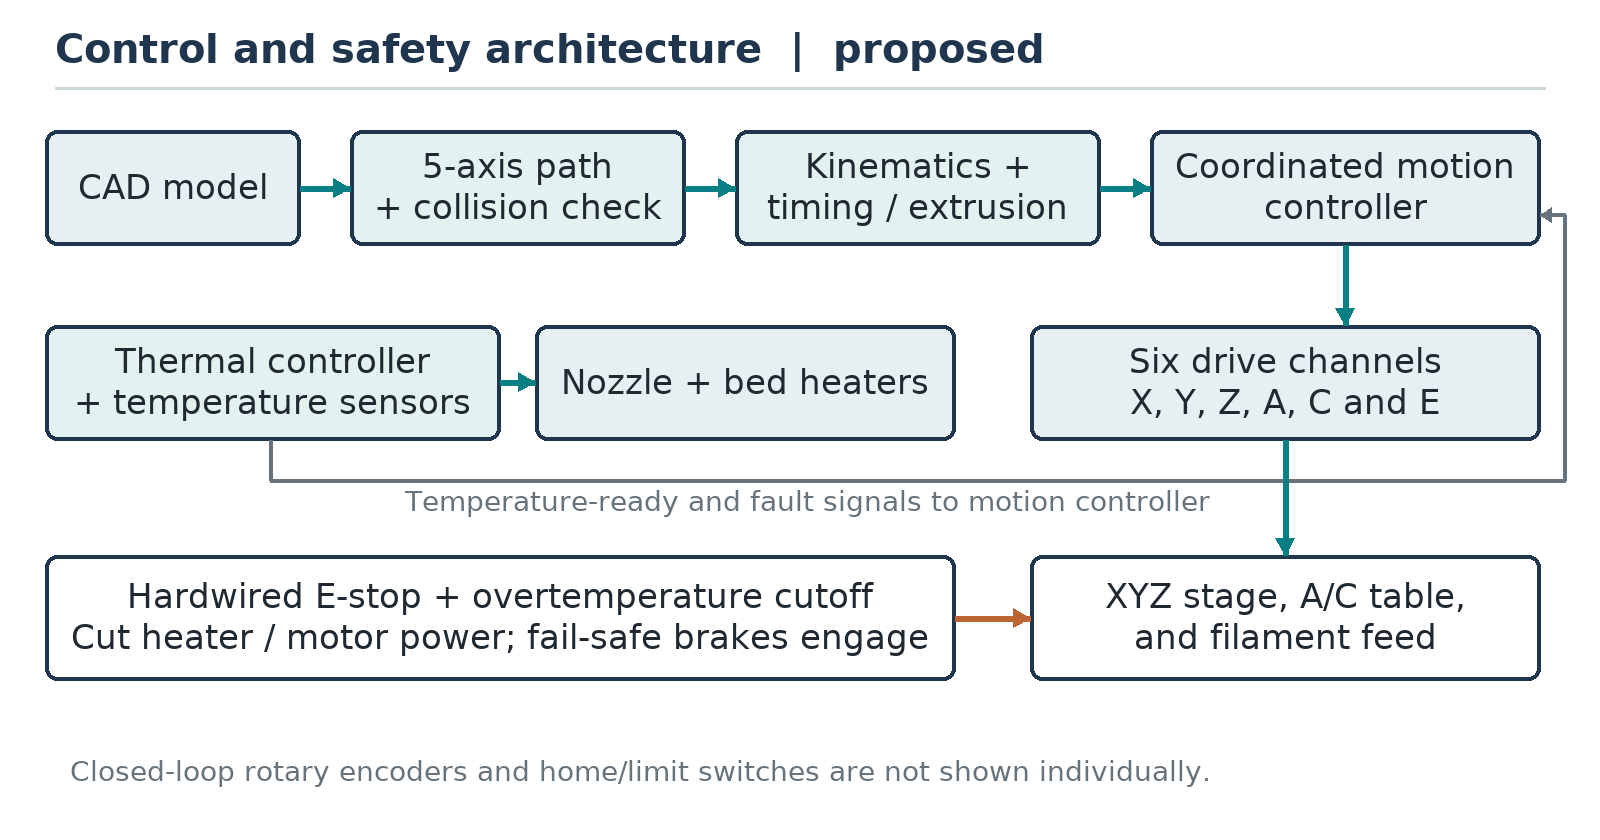
\includegraphics[width=0.96\linewidth,height=\textheight,keepaspectratio]{figures/control_architecture.png}
\caption{Proposed control, heating and hardwired safety architecture. The six drive channels include the
  filament feed, which is not an additional pose degree of freedom.}
\end{figure}

% Avoid separating this heading from its component table.
\Needspace{310pt}
\subsection{Hardware Components, Power and Safety}\label{hardware-components-power-and-safety}

\begingroup
\footnotesize
\setlength{\tabcolsep}{4pt}
\renewcommand{\arraystretch}{1.12}
\begin{longtable}[]{@{}
  >{\raggedright\arraybackslash}p{(\linewidth - 2\tabcolsep) * \real{0.2969}}
  >{\raggedright\arraybackslash}p{(\linewidth - 2\tabcolsep) * \real{0.7031}}@{}}
\caption{Principal proposed hardware; final models and suppliers remain to be selected.}\tabularnewline
\toprule\noalign{}
\begin{minipage}[b]{\linewidth}\raggedright
Subsystem
\end{minipage} & \begin{minipage}[b]{\linewidth}\raggedright
Proposed components and verification need
\end{minipage} \\
\midrule\noalign{}
\endfirsthead
\toprule\noalign{}
\begin{minipage}[b]{\linewidth}\raggedright
Subsystem
\end{minipage} & \begin{minipage}[b]{\linewidth}\raggedright
Proposed components and verification need
\end{minipage} \\
\midrule\noalign{}
\endhead
\bottomrule\noalign{}
\endlastfoot
Mechanical structure & Aluminium frame, linear guides, belts and pulleys, lead screw, bearings, rigid A
  trunnion and C rotary stage; verify stiffness, travel and fasteners. \\
Motion and feed & Six independent drives: X, Y, Z, A, C and E; A/C reducers and output encoders; select
  motors from measured loads and torque--speed curves. \\
Extrusion & 1.75 mm PLA feed mechanism, 0.4 mm nozzle, heater, thermistor, heat-break cooling and
  part-cooling fan. \\
Heated build plate & Approximately 150 mm \ensuremath{\times} 150 mm low-voltage bed, replaceable build
  surface and secure fixture; validate adhesion and retention while tilted. \\
Control and sensing & Coordinated-motion controller, heater controller, independent temperature cutoff,
  X/Y/Z home switches, A/C reference and limit switches, encoder feedback and fault indication. \\
Power and safety & Enclosed 24 V supply, correctly sized protection and wiring, grounded mains enclosure,
  physical guarding, hardwired E-stop and normally engaged A-axis brake. \\
\end{longtable}
\endgroup

For an initial supply estimate, assume 40 W for the nozzle heater, 120 W for the bed, 80 W for
  motors/drivers at the supply input, and 10 W for controls and fans. The total is 250 W, or about 10.4 A
  at 24 V. A 24 V, 15 A (360 W) supply is a preliminary candidate, leaving about 44\% power margin over
  this estimate. Actual peak current, heater resistance, driver losses, wiring temperature and startup
  transients must be checked; the motor figure is an assumed bus input, not the sum of coil ratings.
  Wiring and branch fuses must be selected for actual component ratings and inspected by a qualified
  person.

A hardwired emergency stop must remove power from heaters and motion drives and engage the A brake on
  loss of power; a Z restraint is also required if the screw can back-drive. An independent thermal
  cutoff and heater runaway protection are required in addition to software PID. Guard the moving table
  and belts, insulate hot surfaces, ground the mains enclosure, and provide suitable ventilation. Route
  the bed power and sensor harness in a protected loop sized for the full bounded A/C motion. Test limit
  switches and loss-of-power behaviour before heating or printing. No automatic restart is permitted
  after an emergency stop or unverified loss of position.

\subsection{Toolpath, Extrusion and Integration
  Workflow}\label{toolpath-extrusion-and-integration-workflow}

\begin{enumerate}
\def\labelenumi{\arabic{enumi}.}
\tightlist
\item
  Create the part and fixtures in CAD. Select an achievable geometry and generate a three-axis baseline
  with documented support settings. For the five-axis case, create a geometry-specific inclined or curved
  path with desired part-frame points and outward directions.
\item
  Convert the desired direction to A/C using the stated convention and continuous inverse branch. Compute
  the corresponding nozzle-tip X/Y/Z values with the calibrated pivot and offset. Use \textbf{either}
  this postprocessor transform \textbf{or} a controller's verified rotary-tool-centre-point transform,
  never both.
\item
  Check axis ranges and the full swept volumes of the nozzle tip, heater block, fan shroud, printed
  material accumulated so far, bed, fixtures, frame and cable envelope. Intended nozzle-tip contact with
  the deposition surface is allowed; all unintended contact is rejected. Subdivide moves and evaluate
  interpolated poses, since checking endpoints alone is insufficient.
\item
  First test cold, without filament and at reduced speed; then print with A/C indexed between deposition
  segments; finally attempt a small continuous path that changes A/C and XYZ together. Record actual
  rotary encoder and commanded motion traces. Retraction, safe clearance and cable unwinding are planned
  explicitly.
\end{enumerate}

For a preliminary flow calculation, approximate bead cross-section by \(b\,t\), where bead width
  \(b=0.45\) mm and layer thickness \(t=0.20\) mm. At a part-relative path speed \(v=30\) mm/s, the
  nominal volume flow is \(Q=btv=2.70\) mm\textsuperscript{3}/s. The cross-sectional area of 1.75 mm
  filament is \(A_f=\pi(1.75)^2/4=2.405\) mm\textsuperscript{2}, giving filament speed
  \(v_f=Q/A_f\approx1.12\) mm/s. The rectangular-bead assumption is approximate; real bead shape,
  shrinkage and the hot end's flow limit require calibration.

Extrusion is based on \textbf{part-relative deposited path length}, not simply the distance travelled by
  the nozzle in machine coordinates while the table moves. For a short segment of length \(\ell\),
  command approximately \(\Delta E=bt\ell/A_f\) before empirical flow correction. Segment duration must
  respect the target part-relative speed and every linear, rotary and extruder speed limit; the
  controller must also enforce acceleration and jerk limits and synchronize flow as speed changes.
  Rotary-only travel has no deposition unless explicitly planned. Simulated interpolated motion must
  remain sufficiently close to the intended path, with adequate collision clearance, before any hot run.

\subsection{Calibration and Experimental Validation
  Plan}\label{calibration-and-experimental-validation-plan}

The following tests and acceptance values are \textbf{proposed targets}, not results. Perform
  commissioning in this order, record the instrument and calibration status, and correct deficiencies
  before proceeding.

\begingroup
\footnotesize
\setlength{\tabcolsep}{4pt}
\renewcommand{\arraystretch}{1.12}
\begin{longtable}[]{@{}
  >{\raggedright\arraybackslash}p{(\linewidth - 4\tabcolsep) * \real{0.2237}}
  >{\raggedright\arraybackslash}p{(\linewidth - 4\tabcolsep) * \real{0.4211}}
  >{\raggedright\arraybackslash}p{(\linewidth - 4\tabcolsep) * \real{0.3553}}@{}}
\caption{Proposed commissioning and performance checks.}\tabularnewline
\toprule\noalign{}
\begin{minipage}[b]{\linewidth}\raggedright
Test
\end{minipage} & \begin{minipage}[b]{\linewidth}\raggedright
Proposed procedure
\end{minipage} & \begin{minipage}[b]{\linewidth}\raggedright
Initial acceptance target
\end{minipage} \\
\midrule\noalign{}
\endfirsthead
\toprule\noalign{}
\begin{minipage}[b]{\linewidth}\raggedright
Test
\end{minipage} & \begin{minipage}[b]{\linewidth}\raggedright
Proposed procedure
\end{minipage} & \begin{minipage}[b]{\linewidth}\raggedright
Initial acceptance target
\end{minipage} \\
\midrule\noalign{}
\endhead
\bottomrule\noalign{}
\endlastfoot
Safety and dry motion & Check E-stop, heater cutoff, guards, A brake, Z retention, homing and both rotary
  limits; execute every planned path cold at reduced speed. & All protective functions operate as
  intended; no unintended contact or limit violation. \\
Linear positioning & Measure a 100 mm commanded displacement in both directions on each linear axis for
  five cycles using a suitable independent gauge. & Maximum absolute displacement error \ensuremath{\leq}
  0.20 mm for each axis. \\
Rotary positioning & Independently measure A at \ensuremath{-}25\ensuremath{^\circ}, 0\ensuremath{^\circ}
  and +25\ensuremath{^\circ}, and C at \ensuremath{-}90\ensuremath{^\circ}, 0\ensuremath{^\circ} and
  +90\ensuremath{^\circ}; repeat five times from each approach direction without crossing limits. &
  Maximum absolute angular error \ensuremath{\leq} 1.0\ensuremath{^\circ}; record backlash and each
  approach direction separately. \\
Temperature & With the head and bed at the proposed 200 \ensuremath{^\circ}C and 55 \ensuremath{^\circ}C
  setpoints, compare stable readings over five minutes to independent suitable probes. & Mean error
  within \ensuremath{\pm}5 \ensuremath{^\circ}C at each setpoint; safety cutoffs functional. \\
Planar accuracy & Print five 20 mm calibration cubes at A = C = 0 and measure three principal dimensions
  after cooling. & Each measured dimension within \ensuremath{\pm}0.50 mm of nominal. \\
Five-axis feasibility & Print an indexed inclined feature and a small, simulated continuous curved path.
  Log XYZ/A/C/E commands and A/C encoder motion. & Complete paths without unintended collision or loss of
  adhesion; measurements and any defects recorded. \\
\end{longtable}
\endgroup

\textbf{Support comparison.} Design one overhang bracket that fits the simulated workspace and requires a
  positive, removable support mass in the planar baseline. Make five independent specimens with each
  process on the same machine, using the same PLA batch, nominal part geometry, nozzle diameter,
  temperatures and layer-height settings where physically applicable. A suggested starting feature is an
  approximately 20 mm projecting rib inclined 70\ensuremath{^\circ} from vertical; its exact dimensions
  and paths will be frozen after collision and adhesion checks. Planar prints use a conventional slicer
  with recorded support settings; five-axis prints use a documented, feasible orientation and path.
  Alternate or randomize run order, record any necessary parameter differences, and identify each
  specimen.

For every run, record completion or failure and its cause, print time, actual part dimensions, visible
  defects and separately collected dry support mass. Exclude brims, purges and rafts from the support
  mass, but record them separately. Do not treat a failed print as a zero-support success. For completed
  specimens with measurable supports, calculate:

\[
\text{Support reduction (\%)}=
100\frac{\overline{m}_{\mathrm{planar}}-\overline{m}_{\mathrm{5axis}}}{\overline{m}_{\mathrm{planar}}},
\quad \overline{m}_{\mathrm{planar}}>0.
\]

Report the mean and range, all failures and completion rates for each group, not just the best print. The
  provisional research goal is at least 20\% lower mean support mass for this bracket while achieving at
  least four completed parts out of five in \textbf{each} group and keeping accessible critical
  dimensions within \ensuremath{\pm}0.50 mm of nominal. Five specimens per group are an exploratory
  sample, not enough to establish universal statistical superiority. If the baseline mean is zero or too
  few prints complete, report the comparison as inconclusive and revise the benchmark rather than
  calculating a percentage.

% Keep the work-plan heading with its table when possible.
\Needspace{250pt}
\subsection{Proposed Work Plan and Expected
  Deliverables}\label{proposed-work-plan-and-expected-deliverables}

\begingroup
\footnotesize
\setlength{\tabcolsep}{4pt}
\renewcommand{\arraystretch}{1.12}
\begin{longtable}[]{@{}
  >{\raggedright\arraybackslash}p{(\linewidth - 4\tabcolsep) * \real{0.1867}}
  >{\raggedright\arraybackslash}p{(\linewidth - 4\tabcolsep) * \real{0.4667}}
  >{\raggedright\arraybackslash}p{(\linewidth - 4\tabcolsep) * \real{0.3467}}@{}}
\caption{Indicative twelve-week work plan; timing depends on funding and component
  availability.}\tabularnewline
\toprule\noalign{}
\begin{minipage}[b]{\linewidth}\raggedright
Period
\end{minipage} & \begin{minipage}[b]{\linewidth}\raggedright
Main activities
\end{minipage} & \begin{minipage}[b]{\linewidth}\raggedright
Deliverable or decision
\end{minipage} \\
\midrule\noalign{}
\endfirsthead
\toprule\noalign{}
\begin{minipage}[b]{\linewidth}\raggedright
Period
\end{minipage} & \begin{minipage}[b]{\linewidth}\raggedright
Main activities
\end{minipage} & \begin{minipage}[b]{\linewidth}\raggedright
Deliverable or decision
\end{minipage} \\
\midrule\noalign{}
\endhead
\bottomrule\noalign{}
\endlastfoot
Weeks 1--2 & Review literature; define requirements and compare concepts. & Agreed requirements and
  selection matrix. \\
Weeks 3--4 & Size drives; model the frame, table, pivot and fixtures in CAD; check workspace and FEA. &
  Drawings, load calculations and redesign decisions. \\
Weeks 5--6 & Procure components; assemble frame, drives, table, heater and protected wiring. & Mechanical
  and electrical prototype. \\
Weeks 7--8 & Implement controller and kinematics; tune temperature control; check interlocks and
  calibrate axes. & Safe, homed machine and calibration record. \\
Weeks 9--10 & Generate and simulate paths; perform cold dry runs, planar prints and indexed tests. &
  Verified paths and preliminary print records. \\
Weeks 11--12 & Conduct continuous-path and comparison tests; analyse results and document limitations. &
  Test dataset, final design files and thesis results chapter. \\
\end{longtable}
\endgroup

The bill of materials will be completed after selecting exact components and obtaining current local
  quotations. It should include the frame and fasteners, six motors and compatible drivers, reducers,
  guides, heaters and sensors, controller, supply, protection, wiring, brake, filament and measurement
  equipment, plus a contingency. No prices or procurement outcomes are assumed in this draft. Expected
  outputs are the CAD model, electrical diagram, calibrated kinematic parameters, source/configuration
  for the controller and postprocessor, test records and a final report. Experimental results, discussion
  and final conclusions must be added after the work is performed; none are invented here.


\clearpage
\begin{thebibliography}{9}
\bibitem{iso52900} ISO and ASTM International, \emph{ISO/ASTM 52900:2021, Additive manufacturing ---
  General principles --- Fundamentals and vocabulary}, 2021.
  \url{https://www.iso.org/standard/74514.html}

\bibitem{wulle2017} F. Wulle, D. Coupek, F. Sch\"{a}ffner, A. Verl, F. Oberhofer and T. Maier,
  ``Workpiece and machine design in additive manufacturing for multi-axis fused deposition modeling,''
  \emph{Procedia CIRP}, vol.~60, pp.~229--234, 2017. \url{https://doi.org/10.1016/j.procir.2017.01.046}

\bibitem{shen2018} H. Shen, H. Diao, S. Yue and J. Fu, ``Fused deposition modeling five-axis additive
  manufacturing: machine design, fundamental printing methods and critical process characteristics,''
  \emph{Rapid Prototyping Journal}, vol.~24, no. 3, pp.~548--561, 2018.
  \url{https://doi.org/10.1108/RPJ-05-2017-0096}

\bibitem{isa2019} M. A. Isa and I. Lazoglu, ``Five-axis additive manufacturing of freeform models through
  buildup of transition layers,'' \emph{Journal of Manufacturing Systems}, vol.~50, pp.~69--80, 2019.
  \url{https://doi.org/10.1016/j.jmsy.2018.12.002}

\bibitem{hong2022} F. Hong, S. Hodges, C. Myant and D. E. Boyle, ``Open5x: accessible 5-axis 3D printing
  and conformal slicing,'' in \emph{Extended Abstracts of the 2022 CHI Conference on Human Factors in
  Computing Systems}, article 399, pp.~1--6, 2022. \url{https://doi.org/10.1145/3491101.3519782}

\bibitem{ahlers2019} D. Ahlers, F. Wasserfall, N. Hendrich and J. Zhang, ``3D printing of nonplanar
  layers for smooth surface generation,'' in \emph{2019 IEEE 15th International Conference on Automation
  Science and Engineering (CASE)}, pp.~1737--1743, 2019. \url{https://doi.org/10.1109/COASE.2019.8843116}

\bibitem{nayyeri2022} P. Nayyeri, K. Zareinia and H. Bougherara, ``Planar and nonplanar slicing
  algorithms for fused deposition modeling technology: a critical review,'' \emph{The International
  Journal of Advanced Manufacturing Technology}, vol.~119, pp.~2785--2810, 2022.
  \url{https://doi.org/10.1007/s00170-021-08347-x}

\bibitem{han2025} X. Han, G. Wu, X. Liu, W. Li, X. Song and L. Cui, ``Research on the five-axis
  support-free additive manufacturing method for overhanging parts,'' \emph{Actuators}, vol.~14, no. 2,
  article 99, 2025. \url{https://doi.org/10.3390/act14020099}

\bibitem{tymrak2014} B. M. Tymrak, M. Kreiger and J. M. Pearce, ``Mechanical properties of components
  fabricated with open-source 3-D printers under realistic environmental conditions,'' \emph{Materials \&
  Design}, vol.~58, pp.~242--246, 2014. \url{https://doi.org/10.1016/j.matdes.2014.02.038}
\end{thebibliography}

% End of the complete thesis proposal.
\end{document}
